	\documentclass[tikz]{standalone}
\usepackage{tikz}
\usepackage{graphics}
\usepackage{color}
\usepackage{tikz}
\usetikzlibrary{patterns}
\usetikzlibrary{shapes}
\usetikzlibrary{arrows.meta,arrows}


%%%%%%%%%%%%%%%%%%%%%%%%%%%%%%%%%%%%%%%%%%%%%%%%%%%%%%%%%%%%%%%%%%%%%%%%%%%%%%%%%%%%

%%%  latex --shell-escape CasLevcek.tex

%%%%%%%%%%%%%%%%%%%%%%%%%%%%%%%%%%%%%%%%%%%%%%%%%%%%%%%%%%%%%%%%%%%%%%%%%%%%%%%%%%%%

\usepackage{amssymb} 		%%pour faire lessim
\usepackage{amsmath}		%%pour faire equation*
\usepackage{amsthm} 		%%environnement théorème (!!!)
 \usepackage{array,multirow,makecell}

% \usetikzlibrary{external} % set up externalization

% \tikzexternalize[shell escape=-enable-write18] % activate externalisation

% \tikzset{external/system call={latex \tikzexternalcheckshellescape -halt-on-error
% -interaction=batchmode -jobname "\image" "\texsource" && 
% dvips -o "\image".ps "\image".dvi &&
% ps2eps -l "\image.ps"}}

\begin{document}
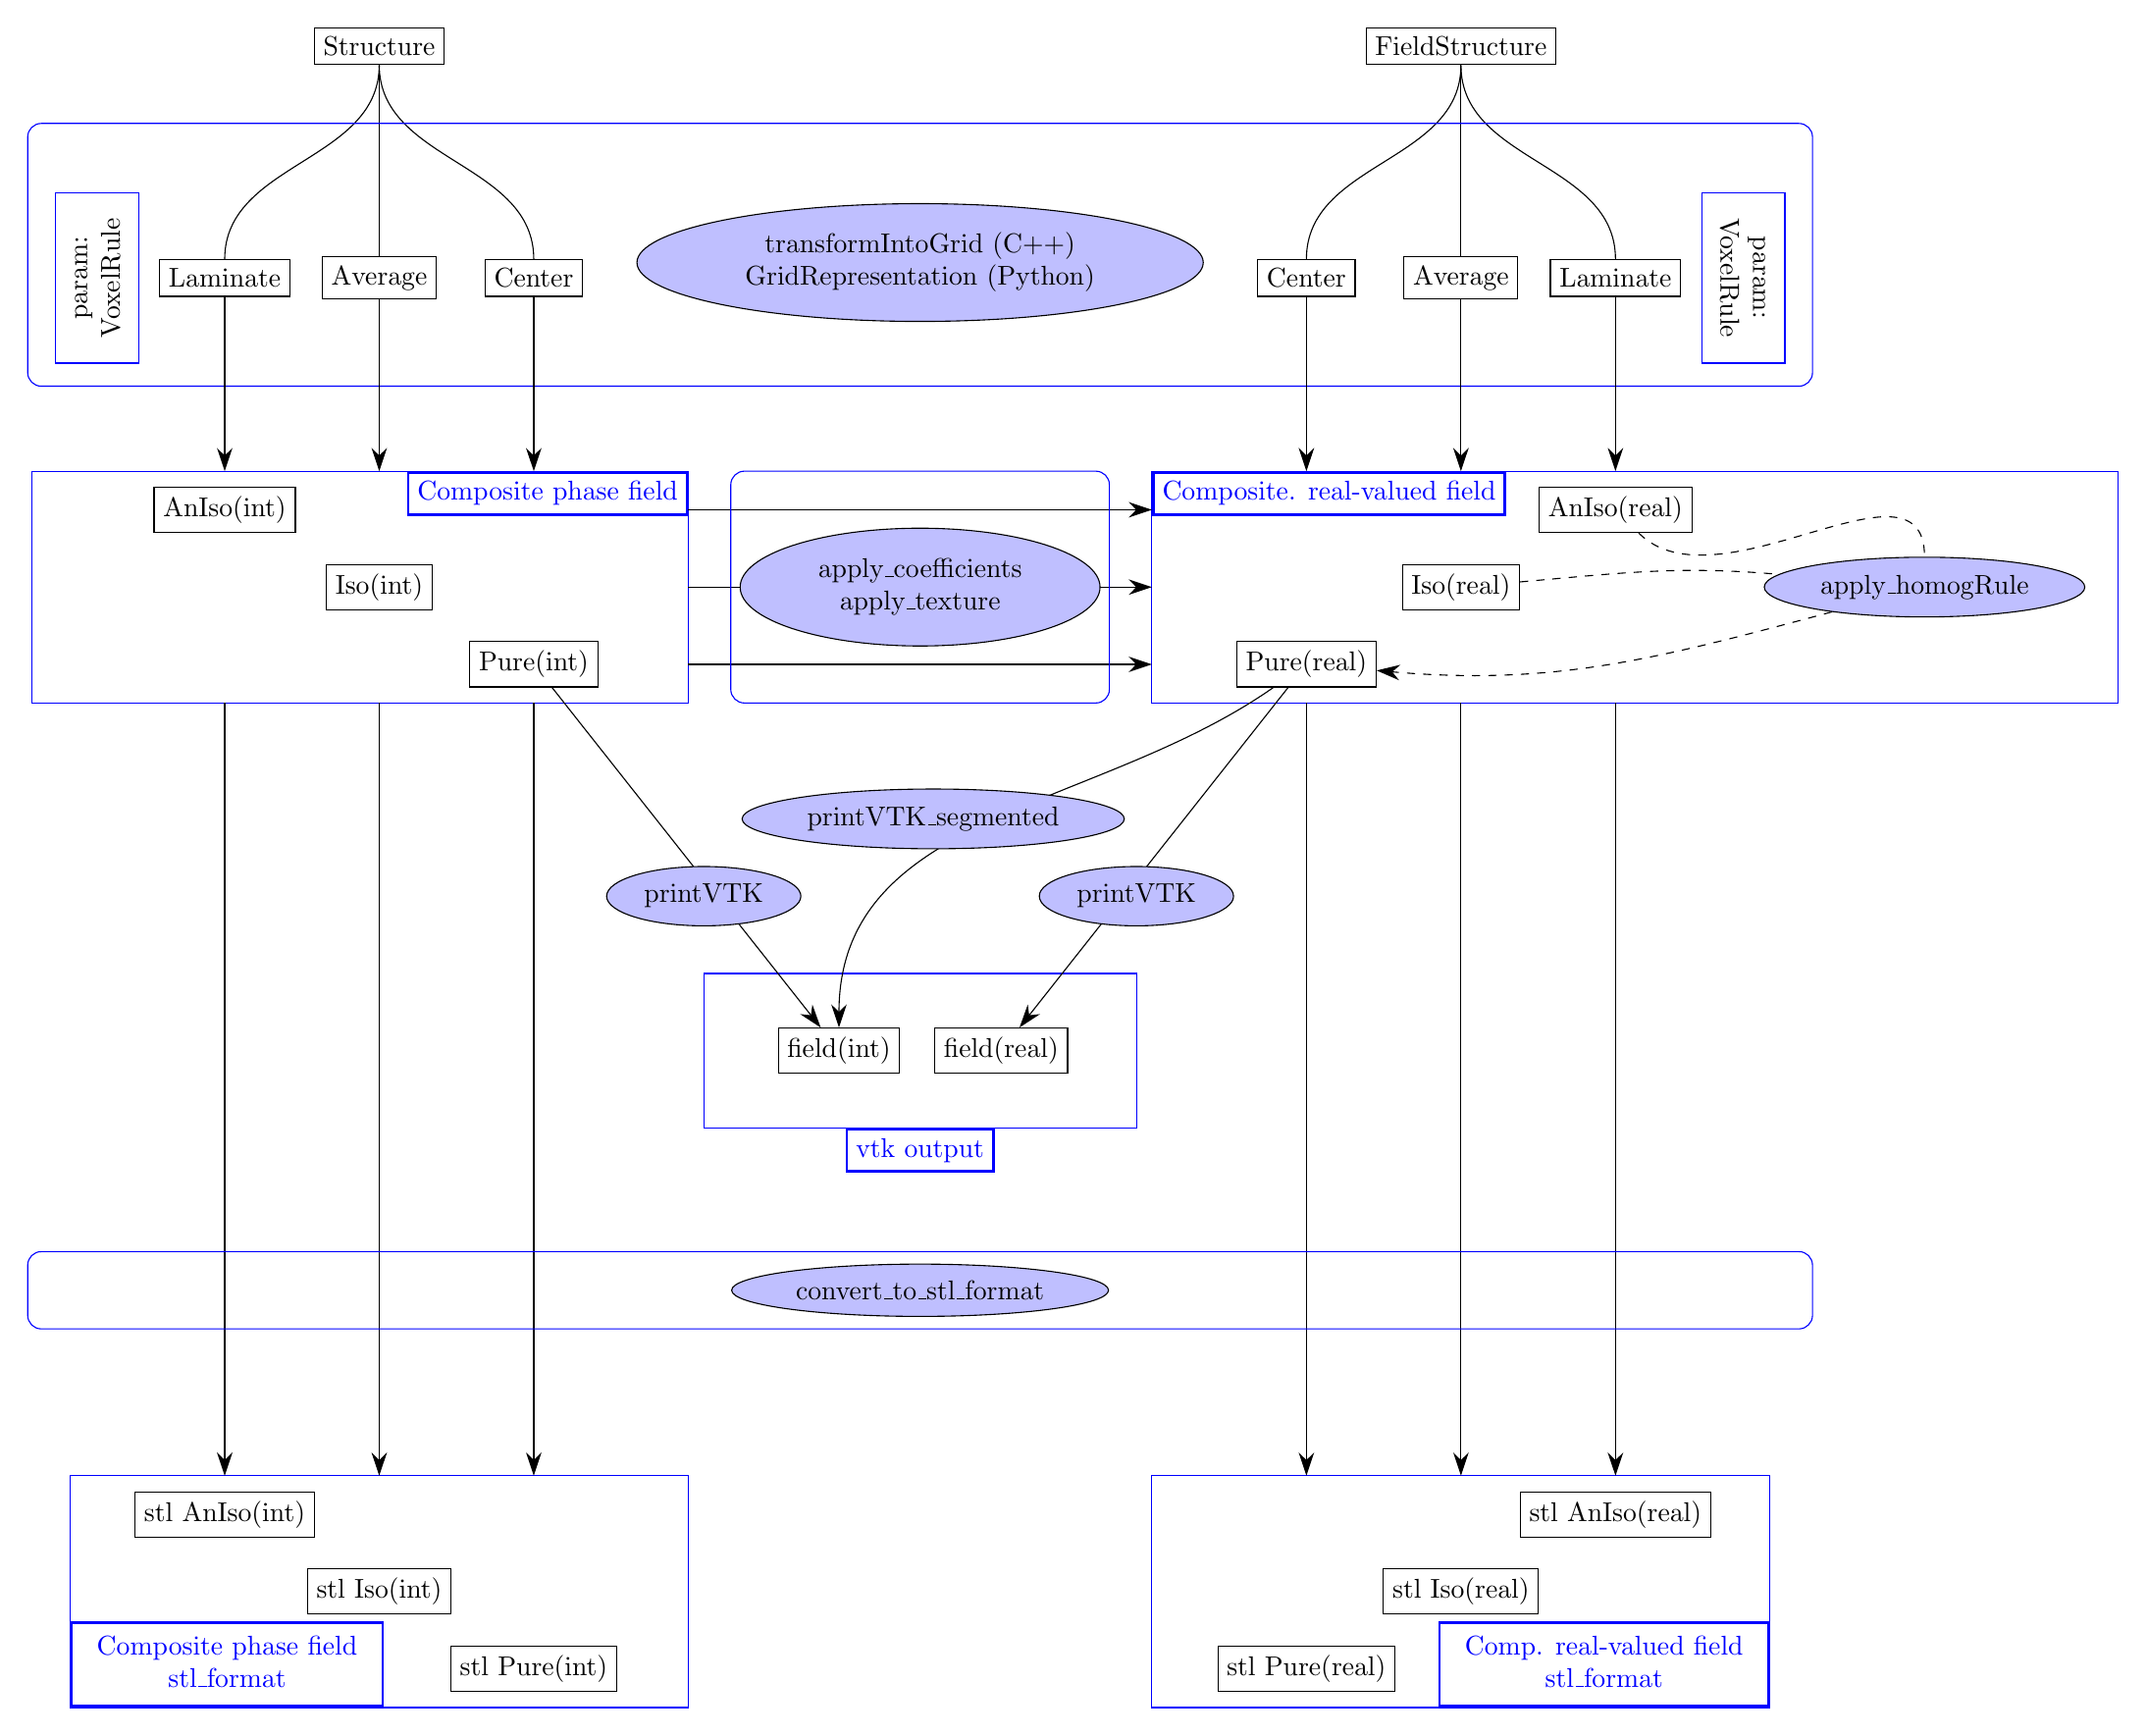
\begin{tikzpicture}[scale = 1]

\def\adist{7};
\def\bdist{2};
\def\cdist{1};
\def\ddist{1};
\def\edist{4};
\def\fdist{13}

\coordinate (CFS) at (\adist, \edist);
\coordinate (CS) at (-\adist, \edist);
\tikzstyle{quadri}=[rectangle,draw]
\tikzstyle{function}=[ellipse,draw,rounded corners=4pt,fill=blue!25]

\node[quadri] (FS) at (CFS) {FieldStructure};
\node[quadri] (S) at (CS) {Structure};

%%% Composite 

\foreach \k in {1, ..., 3}{
	\coordinate (CFS\k) at ( {(\k-2) * \bdist + \adist} , {-\cdist - (4-\k) * \cdist});
	\coordinate(CFSLat\k) at  ( {-2 * \bdist + \adist} , {-\cdist - \k * \cdist});
	\coordinate (CFSBot\k) at  ({(\k-2) * \bdist + \adist} , {-4.5 * \cdist });
	\coordinate (CFSTop\k) at  ( {(\k-2) * \bdist + \adist} , {-1.5 * \cdist});
	\coordinate (CS\k) at  ( {(2-\k) * \bdist - \adist} , {-\cdist - (4-\k) * \cdist});
	\coordinate(CSLat\k) at ( {2 * \bdist - \adist} , {-\cdist - \k * \cdist});
	\coordinate (CSBot\k) at  ( {(2-\k) * \bdist - \adist} , {-4.5 * \cdist });
	\coordinate (CSTop\k) at  ( {(2-\k) * \bdist - \adist} , {-1.5 * \cdist});
}

\draw[color=blue] ({\adist - 2 * \bdist}, {-4.5 * \cdist }) rectangle ({\adist + 4.25 * \bdist}, {-1.5 * \cdist});

\draw[color=blue] ({-\adist - 2.25 * \bdist}, {-4.5 * \cdist }) rectangle ({-\adist + 2 * \bdist}, {-1.5 * \cdist});

\node[quadri] (FS1) at (CFS1) {Pure(real)};
\node[quadri] (FS2) at (CFS2) {Iso(real)};
\node[quadri] (FS3) at (CFS3) {AnIso(real)};

\node[function] (applH) at ({\adist + 3*\bdist}, {-3*\cdist}) {apply\_homogRule};

\draw[dashed] (FS3) edge[out=-45, in=90] (applH);
\draw[dashed] (FS2) edge[out=5, in=175] (applH);
\draw[dashed, ->,-{Stealth[length=3mm, width=2mm]}] (applH) edge[out=-165, in=-5](FS1);


\node[quadri] (S1) at (CS1) {Pure(int)};
\node[quadri] (S2) at (CS2) {Iso(int)};
\node[quadri] (S3) at (CS3) {AnIso(int)};

\node [quadri, color=blue, below left, line width=1] at (-\adist + 2 * \bdist, -1.5 * \cdist) {Composite phase field};

\node [quadri, color=blue, below right, line width=1] at (\adist - 2 * \bdist, -1.5 * \cdist) {Composite. real-valued field};



%%% transfomr into grid


%\node[function] (TS) at (-\adist, 0.6 *\edist) {transformIntoGrid};
%\node[function] (TFS) at (\adist, 0.6 *\edist) {transformIntoGrid};
\node[function] (TSCom) at (0, 0.3 *\edist) {
	\begin{tabular}{c}
	transformIntoGrid (C++)\\
	GridRepresentation (Python)
	\end{tabular}
	};

%\draw(S)--(TSCom);


\foreach \k in {1, ..., 3}{
	\coordinate (CVFS\k) at ( {(\k-2) * \bdist + \adist} , {-\cdist + 0.5 * \edist});
	\coordinate (CVS\k) at  ( {(2-\k) * \bdist - \adist} , {-\cdist  + 0.5 * \edist});
}




\node[quadri]  (VS1) at (CVS1) {Center};
\node[quadri]  (VS2) at (CVS2) {Average};
\node[quadri]  (VS3) at (CVS3) {Laminate};

\node[quadri]  (VFS1) at (CVFS1) {Center};
\node[quadri]  (VFS2) at (CVFS2) {Average};
\node[quadri]  (VFS3) at (CVFS3) {Laminate};

\foreach \k in {1, 2, 3}{
	\draw (S) edge[out=-90,in=90] (VS\k);
	\draw (FS) edge[out=-90,in=90] (VFS\k);
}

%\draw[rounded corners=5pt, color=blue] (-1.65 * \adist, 0.75 *\edist) rectangle (-0.4 * \adist, -0.1 *\edist);
%\draw[rounded corners=5pt, color=blue] (1.65 * \adist, 0.75 *\edist) rectangle (0.4 * \adist, -0.1 *\edist);
\draw[rounded corners=5pt, color=blue] (-1.65 * \adist, 0.75 *\edist) rectangle (1.65 * \adist, -0.1 *\edist);

\node[quadri, color = blue, text=black, below, rotate=90] (wVoxelS) at (-1.6* \adist, {-\cdist  + 0.5 * \edist}) {\begin{tabular}{c} param:\\VoxelRule\end{tabular}};
\node[quadri, color = blue, text=black, below, rotate=270] (wVoxelS) at (1.6* \adist, {-\cdist  + 0.5 * \edist}) {\begin{tabular}{c} param:\\VoxelRule\end{tabular}};


\foreach \k in {1, ..., 3}{
	\draw[->,-{Stealth[length=3mm, width=2mm]}](CSLat\k)--(CFSLat\k);
}

%\node[function] (applyCoeffs) at (0, -2*\cdist) {apply\_coefficients};
\node[function] (applyCoeffs) at (0, -3*\cdist) {
	\begin{tabular}{c}
		apply\_coefficients
		\\
		apply\_texture
	\end{tabular}};

\draw[rounded corners=5pt, color=blue] (-0.35*\adist, -4.5*\cdist) rectangle (0.35*\adist, -1.5*\cdist);

%\node[function] (applyCoeffs) at (0, -4*\cdist) {apply\_coefficients};


\foreach \k in {1, ..., 3}{
	\draw[->,-{Stealth[length=3mm, width=2mm]}] (VS\k)--(CSTop\k);
	\draw[->,-{Stealth[length=3mm, width=2mm]}] (VFS\k)--(CFSTop\k);
}


%%%% print


\node[quadri] (printValue) at (-0.15*\adist, {-9 * \cdist }) {field(int)};
\node[quadri] (printValueF) at (0.15*\adist, {-9 * \cdist }) {field(real)};
\draw[color=blue] (-0.4*\adist, {-10 * \cdist }) rectangle (0.4*\adist, {-8 * \cdist });
\node[quadri, color = blue, line width = 1, below] at (0, -10*\cdist){vtk output};


\draw[->,-{Stealth[length=3mm, width=2mm]}] (S1)--(printValue);
\draw[->,-{Stealth[length=3mm, width=2mm]}] (FS1)--(printValueF);
\draw[->,-{Stealth[length=3mm, width=2mm]}] (FS1) edge[out = 215, in = 90] (printValue);

\node[function] at (-0.4*\adist, - 7 *\cdist) {printVTK};
\node[function] at (0.4*\adist, - 7 *\cdist) {printVTK};
\node[function] (pvtkS) at (0.1\adist, - 6 *\cdist) {printVTK\_segmented};


%%%% stl_format


\foreach \k in {1, ..., 3}{
	\coordinate (CstlFS\k) at ( {(\k-2) * \bdist + \adist} , {-\cdist - (4-\k) * \cdist - \fdist});
	\coordinate (CstlFSTop\k) at ( {(\k-2) * \bdist + \adist} , {-1.5 * \cdist- \fdist});
	\coordinate (CstlS\k) at  ( {(2-\k) * \bdist - \adist} , {-\cdist - (4-\k) * \cdist- \fdist});
	\coordinate (CstlSTop\k) at ( {(2-\k) * \bdist - \adist} , {-1.5 * \cdist- \fdist});
}

\node[quadri] (stlFS1) at (CstlFS1) {stl Pure(real)};
\node[quadri] (stlFS2) at (CstlFS2) {stl Iso(real)};
\node[quadri] (stlFS3) at (CstlFS3) {stl AnIso(real)};

\node[quadri] (stlS1) at (CstlS1) {stl Pure(int)};
\node[quadri] (stlS2) at (CstlS2) {stl Iso(int)};
\node[quadri] (stlS3) at (CstlS3) {stl AnIso(int)};

\draw[color=blue] ({\adist - 2 * \bdist}, {-4.5 * \cdist - \fdist}) rectangle ({\adist + 2 * \bdist}, {-1.5 * \cdist- \fdist});

\draw[color=blue] ({-\adist - 2 * \bdist}, {-4.5 * \cdist - \fdist}) rectangle ({-\adist + 2 * \bdist}, {-1.5 * \cdist- \fdist});

\node [quadri, color=blue, above right, line width=1] at (-\adist - 2 * \bdist,  {-4.5 * \cdist - \fdist}) {\begin{tabular}{c} Composite phase field \\  stl\_format \end{tabular}};

\node [quadri, color=blue, above left, line width=1] at (\adist + 2 * \bdist,  {-4.5 * \cdist - \fdist}) {\begin{tabular}{c} Comp. real-valued field \\  stl\_format \end{tabular}};

%\foreach \k in {1, ..., 3}{
%	\draw[->,-{Stealth[length=3mm, width=2mm]}](stlS\k)--(stlFS\k);
%}

%\node[function] (applyCoeffs) at (0, -\fdist -2*\cdist) {apply\_coefficients};
%\node[function] (applyCoeffs) at (0, -\fdist -3*\cdist) {apply\_coefficients};
%\node[function] (applyCoeffs) at (0, -\fdist -4*\cdist) {apply\_coefficients};

\foreach \k in {1, ..., 3}{
	\draw[->,-{Stealth[length=3mm, width=2mm]}] (CSBot\k)--(CstlSTop\k);
	\draw[->,-{Stealth[length=3mm, width=2mm]}] (CFSBot\k)--(CstlFSTop\k);
}

\draw[rounded corners=5pt, color=blue] (-1.65 * \adist, - 3.5 * \cdist - 0.7 * \fdist) rectangle (1.65 * \adist, - 2.5* \cdist - 0.7 * \fdist);

\node[function](convertSTL) at (0, - 3 * \cdist - 0.7 * \fdist) {convert\_to\_stl\_format};

\end{tikzpicture}
\end{document}
